% This is LLNCS.DEM the demonstration file of
% the LaTeX macro package from Springer-Verlag
% for Lecture Notes in Computer Science,
% version 2.4 for LaTeX2e as of 16. April 2010
%
\documentclass{llncs}
%
\usepackage{amsmath}
\usepackage{amssymb}
\usepackage{tikz}
\usepackage[linesnumbered,ruled]{algorithm2e}

\newcounter{instr}
\newcommand{\ninstr}{\refstepcounter{instr}\theinstr.}

\begin{document}

\title{Species delimitation}

\titlerunning{Species delimitation}

\author{Tom\'{a}\v{s} Flouri\inst{1} \and Paschalia Kapli\inst{1} \and Sarah Lutteropp\inst{1}}
\authorrunning{Tom\'{a}\v{s} Flouri et al.} % abbreviated author list
\institute{Heidelberg Institute of Theoretical Studies}

\maketitle

\begin{abstract}
An explanation of the Bayesian approach for PTP.\@
\end{abstract}

\section{Allowed Moves}

In order to change a delimitation in the MCMC steps, we randomly select one of two possible moves (see Fig.~\ref{fig:moves}).

\begin{figure}[h!]
\centering
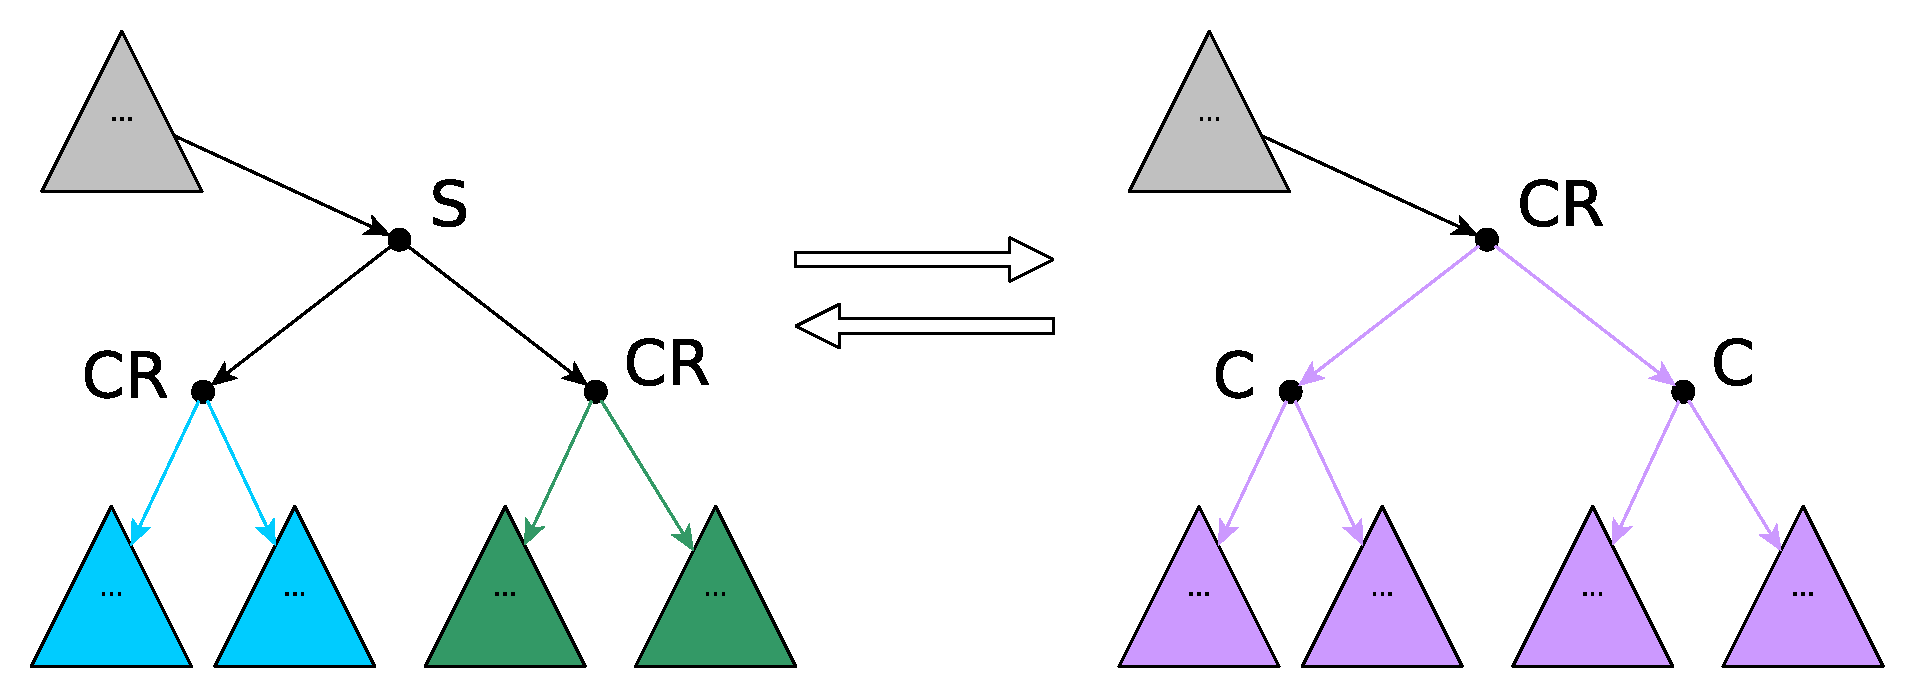
\includegraphics[scale=0.4]{images/moves.pdf}
\caption{Allowed moves in the Bayesian steps. The black edges belong to the speciation part, the colored edges are within species. The node label ``S'' means that a node is a speciation event, whereas the labels ``C'' and ``CR'' mean that a node is a coalescent event. The difference between ``C'' and ``CR'' is that ``CR'' stands for a coalescent root node, i.e. the MRCA of a species.}
\label{fig:moves}
\end{figure}

\bibliographystyle{splncs03}
\bibliography{delimit}
\end{document}
